%% Преамбула TeX-файла

% 1. Стиль и язык
\documentclass[utf8x, 12pt]{G7-32} % Стиль (по умолчанию будет 14pt)

% Остальные стандартные настройки убраны в preamble.inc.tex.
% russian language
\usepackage[utf8]{inputenc}
\usepackage[T2A]{fontenc}
\usepackage[english,russian]{babel}

% searchable and copyable
\usepackage{cmap}

% Times New Roman
\usepackage{pscyr}
\renewcommand{\rmdefault}{ftm}

% Margins
\usepackage{geometry}
\geometry{left=30mm}
\geometry{right=10mm}
\geometry{top=20mm}
\geometry{bottom=20mm}

% Titles
\usepackage{titlesec}
\titlespacing*{\chapter}{\parindent}{-30pt}{21pt}
\titlespacing*{\section}{\parindent}{*2}{*2}
\titlespacing*{\subsection}{\parindent}{*2}{*2}
\titleformat{\chapter}{\LARGE\bfseries}{\thechapter}{18pt}{\LARGE\bfseries}
\titleformat{\section}{\Large\bfseries}{\thesection}{16pt}{\Large\bfseries}

% Spacing
\usepackage{setspace}
\usepackage{indentfirst}
\setlength{\parindent}{1.25cm}
\linespread{1.25}

% Links
\usepackage[unicode, pdftex]{hyperref}
\def\UrlBreaks{\do\/\do-\do\_}
\usepackage[nottoc]{tocbibind} % for bib link

% Listings
\usepackage{listings}
\usepackage[newfloat]{minted}
\usepackage{verbatim}
\usepackage[framemethod=tikz]{mdframed}

\mdfdefinestyle{mymdstyle}{
    innerleftmargin=0mm,
    innerrightmargin=0mm,
    innertopmargin=-4pt,
    innerbottommargin=-9pt,
    splittopskip=\baselineskip,
    hidealllines=true,
    middleextra={
      \node[anchor=west] at (O|-P)
        {\lstlistingname~\thelstlisting~(продолжение)};
        },
    secondextra={
      \node[anchor=west] at (O|-P)
        {\lstlistingname~\thelstlisting~(продолжение)};},
}

\surroundwithmdframed[style=mymdstyle]{lstlisting}
\newmdenv[style=mymdstyle]{mdlisting}

\newcommand{\mylisting}[4] {
    \noindent
    \begin{minipage}{\linewidth}
        \captionsetup{justification=raggedright,singlelinecheck=off}
        \begin{lstinputlisting}[
            caption={#1},
            label={lst:#2},
            linerange={#3}
        ]{../../src/#4}
        \end{lstinputlisting}
    \end{minipage}
}

\newcommand{\mybreaklisting}[4]{
    \begin{mdlisting}
        \captionsetup{justification=raggedright,singlelinecheck=off}
        \lstinputlisting[label=lst:#2, caption=#1,
        linerange=#3]{../../src/#4}
    \end{mdlisting}
}

% Images
\usepackage{graphicx}
\newcommand{\scheme}[4] {
	\begin{figure}[ht!]
		\center{
            \includegraphics[width=#1]{../data/schemes/#2}
            \caption{#3}
            \label{scheme:#4}
        }
	\end{figure}
}

\newcommand{\img}[4] {
	\begin{figure}[ht!]
		\center{
            \includegraphics[height=#1]{../data/img/#2}
            \caption{#3}
            \label{img:#4}
        }
	\end{figure}
}

% Captions
\usepackage[figurename=Рисунок,labelsep=endash,
            justification=centering]{caption}
\usepackage{hyphenat}

% Lists
\usepackage{enumitem}
\renewcommand{\labelitemi}{$-$}
\setlist{nosep, leftmargin=\parindent, wide}

% Comments
\usepackage{comment}

% Text
\usepackage{amstext}
\usepackage{ulem}
\renewcommand{\ULdepth}{1.5pt}

% Formulas
\usepackage{amsmath}

% Tabulars
\usepackage{threeparttable}
\usepackage{csvsimple}
\usepackage{longtable,ltcaption,booktabs}
\newcommand{\specialcell}[2][c]{%
  \begin{tabular}[#1]{@{}c@{}}#2\end{tabular}}

\newcommand{\csvtable}[3]{
    \begin{table}[h]
        \begin{center}
        \begin{threeparttable}
            \captionsetup{format=hang,justification=raggedright,
                          singlelinecheck=off}
            \caption{\label{tab:#1}#2}
            \begin{tabular}{|r|r|r|r|}
                \hline
                \bfseries $\alpha$ & \bfseries $p$ &
                \bfseries Число итераций & \bfseries Ошибка 
                \csvreader{../data/csv/#3.csv}{}
                {\\\hline \csvcoli&\csvcolii&\csvcoliii&\csvcoliv}
                \\\hline
            \end{tabular}
        \end{threeparttable}
        \end{center}
    \end{table} 
}


% Настройки листингов.
\ifPDFTeX
% russian language support by listings
% replace sign to text
\lstset{
	literate=
	{а}{{\selectfont\char224}}1
	{б}{{\selectfont\char225}}1
	{в}{{\selectfont\char226}}1
	{г}{{\selectfont\char227}}1
	{д}{{\selectfont\char228}}1
	{е}{{\selectfont\char229}}1
	{ё}{{\"e}}1
	{ж}{{\selectfont\char230}}1
	{з}{{\selectfont\char231}}1
	{и}{{\selectfont\char232}}1
	{й}{{\selectfont\char233}}1
	{к}{{\selectfont\char234}}1
	{л}{{\selectfont\char235}}1
	{м}{{\selectfont\char236}}1
	{н}{{\selectfont\char237}}1
	{о}{{\selectfont\char238}}1
	{п}{{\selectfont\char239}}1
	{р}{{\selectfont\char240}}1
	{с}{{\selectfont\char241}}1
	{т}{{\selectfont\char242}}1
	{у}{{\selectfont\char243}}1
	{ф}{{\selectfont\char244}}1
	{х}{{\selectfont\char245}}1
	{ц}{{\selectfont\char246}}1
	{ч}{{\selectfont\char247}}1
	{ш}{{\selectfont\char248}}1
	{щ}{{\selectfont\char249}}1
	{ъ}{{\selectfont\char250}}1
	{ы}{{\selectfont\char251}}1
	{ь}{{\selectfont\char252}}1
	{э}{{\selectfont\char253}}1
	{ю}{{\selectfont\char254}}1
	{я}{{\selectfont\char255}}1
	{А}{{\selectfont\char192}}1
	{Б}{{\selectfont\char193}}1
	{В}{{\selectfont\char194}}1
	{Г}{{\selectfont\char195}}1
	{Д}{{\selectfont\char196}}1
	{Е}{{\selectfont\char197}}1
	{Ё}{{\"E}}1
	{Ж}{{\selectfont\char198}}1
	{З}{{\selectfont\char199}}1
	{И}{{\selectfont\char200}}1
	{Й}{{\selectfont\char201}}1
	{К}{{\selectfont\char202}}1
	{Л}{{\selectfont\char203}}1
	{М}{{\selectfont\char204}}1
	{Н}{{\selectfont\char205}}1
	{О}{{\selectfont\char206}}1
	{П}{{\selectfont\char207}}1
	{Р}{{\selectfont\char208}}1
	{С}{{\selectfont\char209}}1
	{Т}{{\selectfont\char210}}1
	{У}{{\selectfont\char211}}1
	{Ф}{{\selectfont\char212}}1
	{Х}{{\selectfont\char213}}1
	{Ц}{{\selectfont\char214}}1
	{Ч}{{\selectfont\char215}}1
	{Ш}{{\selectfont\char216}}1
	{Щ}{{\selectfont\char217}}1
	{Ъ}{{\selectfont\char218}}1
	{Ы}{{\selectfont\char219}}1
	{Ь}{{\selectfont\char220}}1
	{Э}{{\selectfont\char221}}1
	{Ю}{{\selectfont\char222}}1
	{Я}{{\selectfont\char223}}1
}

% set asm listing style
\lstset{
	language={Go},
	backgroundcolor=\color{white},
	basicstyle=\footnotesize\ttfamily,
	keywordstyle=\color{blue},
	stringstyle=\color{red},
	commentstyle=\color{gray},
	numbers=left,
	numberstyle=\footnotesize,
	stepnumber=1,
	numbersep=5pt,
	frame=single,
	tabsize=4,
	captionpos=t,
	breaklines=true
}

\captionsetup[lstlisting]{format=hang, justification=justified}

\else
\usepackage{local-minted}
\fi

% Полезные макросы листингов.
% Любимые команды
\newcommand{\Code}[1]{\textbf{#1}}


\begin{document}

\frontmatter 

% \begin{titlepage}
% 	\centering
% 	{\scshape\LARGE МГТУ им. Баумана \par}
% 	\vspace{3cm}
% 	{\scshape\Large Лабораторная работа №4\par}
% 	\vspace{0.5cm}
% 	{\scshape\Large По курсу: "Анализ алгоритмов"\par}
% 	\vspace{1.5cm}
% 	{\huge\bfseries Параллельное умножение матриц\par}
% 	\vspace{2cm}
% 	\Large Работу выполнила: Оберган Татьяна, ИУ7-55Б\par
% 	\vspace{0.5cm}
% 	\LargeПреподаватели:  Волкова Л.Л., Строганов Ю.В.\par

% 	\vfill
% 	\large \textit {Москва, 2019} \par
% \end{titlepage}


% НАЧАЛО ТИТУЛЬНОГО ЛИСТА
\noindent \begin{minipage}{0.15\textwidth}
	
\includegraphics[width=\linewidth]{b_logo}
\end{minipage}
\noindent\begin{minipage}{0.9\textwidth}\centering
	\textbf{Министерство науки и высшего образования Российской Федерации}\\
	\textbf{Федеральное государственное бюджетное образовательное учреждение высшего образования}\\
	\textbf{«Московский государственный технический университет имени Н.Э.~Баумана}\\
	\textbf{(национальный исследовательский университет)»}\\
	\textbf{(МГТУ им. Н.Э.~Баумана)}
\end{minipage}

\noindent\rule{18cm}{3pt}
\newline
\noindent ФАКУЛЬТЕТ $\underline{\text{«Информатика и системы управления»}}$ \newline
\noindent КАФЕДРА $\underline{\text{«Программное обеспечение ЭВМ и информационные технологии»}}$\newline


\begin{center}
	\noindent\begin{minipage}{1.2\textwidth}\centering
		\textbf{ОТЧЕТ ПО ЛАБОРАТОРНОЙ РАБОТЕ №7}\newline
		\textbf{По курсу: "Анализ алгоритмов"}\newline\newline\newline
	\end{minipage}
\end{center}




\noindent ~~Студент $\underline{\text{~~~~~~~~~~~~~~~~~~~~~~~~~~~~~~~~~Сукочева Алис~~~~~~~~~~~~~~~~~~~~~~~~~~~~~~~~~~~~~~~~~~~~~~~}}$

\noindent ~~Группа $\underline{\text{~~~~~~~~~~~~~~~~~~~~~~~~~~~~~~~~~~~~~~ИУ7-53Б~~~~~~~~~~~~~~~~~~~~~~~~~~~~~~~~~~~~~~~~~~~~~~~~~~~~}}$

\noindent ~~Название предприятия $\underline{\text{~~~~~~~~МГТУ им. Н. Э. Баумана, каф. ИУ7~~~~~~~~~~~~~~~~~~~~~~}}$

\noindent ~~Тема $\underline{\text{~~~~~~~~~~~~~~~~~~~~~~~~~~~~~~~~~~~~~~~~~Поиск в словаре.~~~~~~~~~~~~~~~~~~~~~~~~~~~~~~~~~~~~~~~~~~~~~~~~~~~}}$\newline


\noindent\begin{tabular}{lcc}
	Студент: ~~~~~~~~~~~~~~~~~~~~~~~~~~~~~~~~~~~~~~~~~~~~~~~~~~~~~~~~ & $\underline{\text{~~~~~~~~~~~~~~~~}}$ & $\underline{\text{~~Сукочева А.~~}}$       \\
	                                                                  & \footnotesize подпись, дата           & \footnotesize Фамилия, И.О.                \\
	%& &  \\
	Преподаватель:                                                    & $\underline{\text{~~~~~~~~~~~~~~~~}}$ & $\underline{\text{~~~~Волкова Л.Л.~~~}}$   \\
	                                                                  & \footnotesize подпись, дата           & \footnotesize Фамилия, И. О.               \\
	Преподаватель:                                                    & $\underline{\text{~~~~~~~~~~~~~~~~}}$ & $\underline{\text{~~~~Строганов Ю.В.~~~}}$ \\
	                                                                  & \footnotesize подпись, дата           & \footnotesize Фамилия, И. О.               \\
\end{tabular}


\begin{center}
	\vfill
	Москва~---~\the\year
	~г.
\end{center}

\thispagestyle{empty}
% КОНЕЦ ТИТУЛЬНОГО ЛИСТА

\tableofcontents

\newpage
\addcontentsline{toc}{chapter}{Введение}

\chapter*{Введение}
Многие задачи требуют огромных вычислительных мощностей, но даже суперкомпьютеры не всегда справляются с поставленными задачами.
Вычислительные конвейеры предоставляют возможность распараллелить исходный алгоритм для оптимального использования системных ресурсов.
Вычислительные конвейеры используются в процессорах для ускорения выполнения инструкций.

Целью данной работы является разработка программы, которая реализует два способа реализации
вычислительного конвейера: линейный и с использованием параллельных вычислений.

Для достижения поставленной цели необходимо выполнить следующее:
\begin{itemize}
	\item рассмотреть методологию конвейерной разработки;
	\item рассмотреть способы распараллеливания конвейерных вычислений;
	\item привести схемы реализации конвейера;
	\item определить средства программной реализации;
	\item реализовать рассматриваемые способы реализации вычислительного конвейера;
	\item протестировать разработанное ПО;
	\item провести модульное тестирование всех реализаций алгоритмов;
	\item оценить реализацию алгоритмов по времени и памяти.
\end{itemize}

\mainmatter % это включает нумерацию глав и секций в документе ниже

\chapter{ Аналитический раздел}
\label{cha:analysis}

\section{Некоторые теоретические сведения}

Для начала нужно ввести собственно понятие матрицы.

\textit{Матрица} -- объект, записываемый в виде прямоугольной таблицы элементов,
которая представляет собой совокупность строк и столбцов, на пересечении которых находятся её элементы (формула \ref{eq:ref1}).

\begin{equation}
	A = \left(
	\begin{array}{cccc}
			a_{11} & a_{12} & \ldots & a_{1n} \\
			a_{21} & a_{22} & \ldots & a_{2n} \\
			\vdots & \vdots & \ddots & \vdots \\
			a_{n1} & a_{n2} & \ldots & a_{nn}
		\end{array}
	\right)
	\label{eq:ref1}
\end{equation}

\textit{Произведение матриц} AB состоит из всех возможных комбинаций скалярных произведений 
вектор-строк матрицы A и вектор-столбцов матрицы B (рис. \ref{fg:ref2}).

\begin{figure}[ht!]
	\centering{
		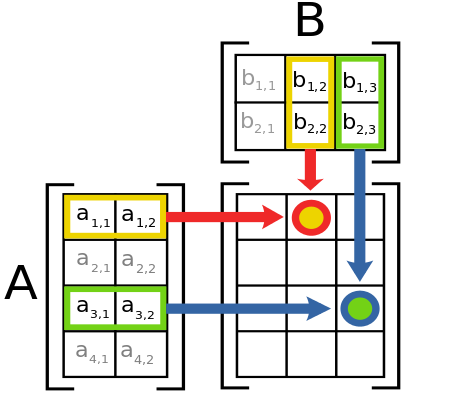
\includegraphics[width=0.5\textwidth]{img/matrix_mult.png}
		\caption{Произведение матриц}
		\label{fg:ref2}}
\end{figure}

Операция умножения двух матриц выполнима только в том случае, если число столбцов в первой матрице равно числу строк во второй.

\section{Стандартный алгоритм умножения матриц}

Допустим имеется матрицы A (формула \ref{eq:ref1}) и B (формула \ref{eq:ref2})

\begin{equation}
	B = \left(
	\begin{array}{cccc}
			b_{11} & b_{12} & \ldots & b_{1n} \\
			b_{21} & b_{22} & \ldots & b_{2n} \\
			\vdots & \vdots & \ddots & \vdots \\
			b_{n1} & b_{n2} & \ldots & b_{nn}
		\end{array}
	\right)
	\label{eq:ref2}
\end{equation}

Матрица C = AB будет размерностью $l \times n$, 
где матрица A размерностью $l \times m$, а матрица B $m \times n$
Тогда каждый элемент матрицы C выражается формулой (\ref{eq:ref3})

\begin{equation}
	\begin{array}{cc}
		c_{ij} = \sum\limits_{r=1}^m a_{ir}b_{ri} & (i=1,2,\dots l; j=1,2,\dots n)
	\end{array}
	\label{eq:ref3}
\end{equation}

\section{Умножение матриц по Винограду}

Каждый элемент в матрице C, которая является результатом умножения двух матриц,
представляет собой скалярное произведение соответствующих строки и столбца исходных матриц. 
В алгоритме умножение матриц по Винограду предложено сделать предварительную обработку,
позволяющую часть работы выполнить заранее.

Рассмотрим два вектора V (формула \ref{eq:ref4}) и W (формула \ref{eq:ref5}).

\begin{equation}
	V = (v_1, v_2, v_3, v_4)
	\label{eq:ref4}
\end{equation}

\begin{equation}
	W = (w_1, w_2, w_3, w_4)
	\label{eq:ref5}
\end{equation}

Их скалярное произведение равно  \ref{eq:ref6}.

\begin{equation}
	V * W = v_1w_1 + v_2w_2 + v_3w_3 + v_4w_4
	\label{eq:ref6}
\end{equation}

Равенство \ref{eq:ref6} можно записать в виде \ref{eq:ref7}.

\begin{equation}
	\begin{array}{l}
		V * W = (v_1 + w_2)(v_2 + w_1) + (v_3 + w_4)(v_4 + w_3) - \\
		\quad \quad \quad v_1v_2 - v_3v_4 - w_1w_2 - w_3w_4
	\end{array}
	\label{eq:ref7}
\end{equation}

Выражение в правой части равенства \ref{eq:ref7} допускает предварительную обработку:
его части можно вычислить заранее и запомнить для каждой строки первой матрицы и для каждого столбца второй. На практике это означает,
что над предварительно обработанными элементами нам придется выполнять лишь первые два умножения и последующие пять сложений, а
также дополнительно два сложения.

\section{Вывод}

Были рассмотрены основополагающие материалами, которые в дальнейшем потребуются при реализации алгоритмов умножения матриц.  




\chapter{ Констукторский раздел}
\label{cha:design}

В данном разделе мы рассмотрим схемы алгоритмов сортировки.

На рис. \ref{d:ref1} представлена схема алгоритма сортировки пузырьком.

\begin{figure}[ht!]
	\centering{
		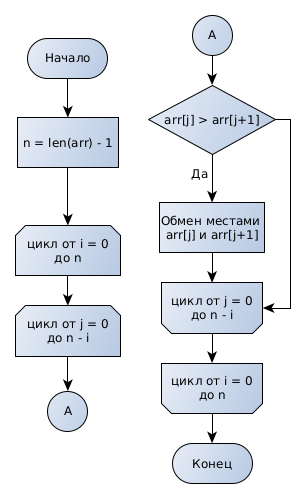
\includegraphics[width=0.5\textwidth]{img/unnamed0.png}
		\caption{Схема алгоритма сортировки пузырьком}
		\label{d:ref1}}
\end{figure}

На рис. \ref{d:ref2} представлена схема алгоритма сортировки вставками.

\begin{figure}[ht!]
	\centering{
		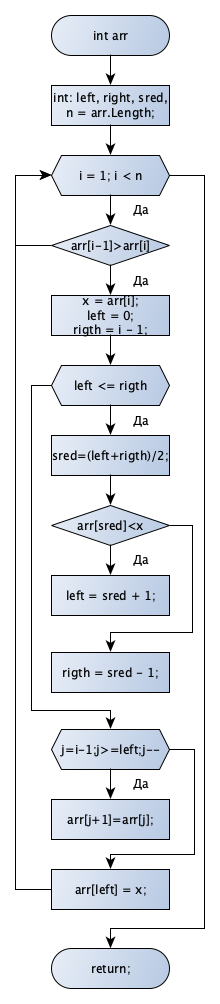
\includegraphics[width=0.5\textwidth]{img/unnamed1.png}
		\caption{Схема алгоритма сортировки вставками}
		\label{d:ref2}}
\end{figure}

На рис. \ref{d:ref3} представлена схема алгоритма quicksort.

\begin{figure}[ht!]
	\centering{
		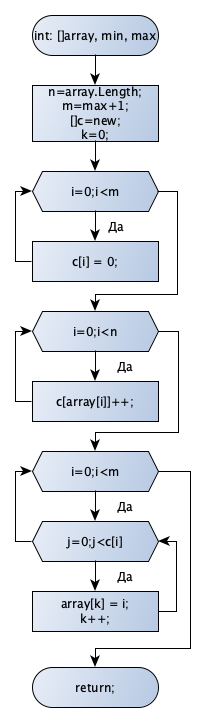
\includegraphics[width=0.5\textwidth]{img/unnamed2.png}
		\caption{Схема алгоритма сортировки quicksort}
		\label{d:ref3}}
\end{figure}


\section{Вывод}

В данном разделе были рассмотрены схемы (рис. \ref{d:ref1} - \ref{d:ref3}) алгоритмов сортировки.







\chapter{ Технологический раздел}
\label{cha:design}

\section{Выбор ЯП}

В данной лабораторной работе использовался язык программирования - python \cite{bib1}.
Данный язык простой и понятный, также я знакома с ним.
Поэтому данный язык был выбран. 
В качестве среды разработки я использовала Visual Studio Code \cite{bib2}, т.к. считаю его достаточно удобным и легким.
Visual Studio Code подходит не только для  Windows \cite{bib3}, но и для Linux \cite{bib4}, это еще одна причина, по которой я выбрала VS code, т.к. у меня установлена ОС Ubuntu 18.04.4 \cite{bib5}.

\section{Требования к программному обеспечению}

Входными данными являются

На выходе

\section{Сведения о модулях программы}

Данная программа разбита на модули:

\begin{itemize}
	\item main.py - Файл, содержащий точку входа в программу. В нем происходит общение с пользователем и вызов алгоритмов;
\end{itemize}

На листингах 3.1-3.6 представлены 

% \begin{lstlisting}[label=some-code,caption=Главная функция main]
% \end{lstlisting}

\section{Тестирование}

В данном разделе будет приведена таблица 
% \ref{table:ref1}, в которой четко отражено тестирование программы. ы

\section{Вывод}

В данном разделе были ...
\chapter{Экспериментальная часть}

В данном разделе будет произведено сравнение двух алгоритмов:

\begin{enumerate}
	\item полный перебор;
	\item муравьиный алгоритм.
\end{enumerate}

\section{Сравнение времени работы муравьиного алгоритма и полного перебора}

Для сравнения возьмем 8 массивов городов размерностью
$[$3, 4, 5, 6, 7, 8, 9, 10$]$.
Воспользуемся усреднением массового эксперимента.

Результат сравнения муравьиного алгоритма и полного перебора представлен на рис. \ref{ref:time}.

\begin{figure}[ht!]
	\centering{
		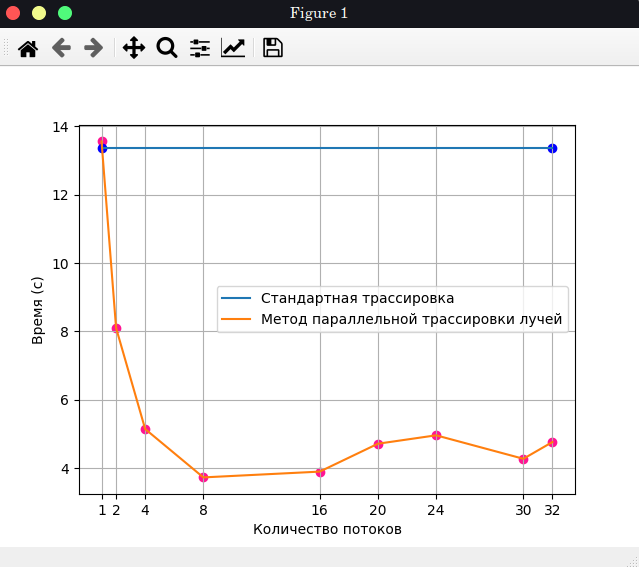
\includegraphics[width=0.8\textwidth]{time.png}
		\caption{Время работы муравьиного алгоритма и полного перебора}
		\label{ref:time}}
\end{figure}

По результатам эксперимента видно, что время испольнения муравьиного алгоритма
значительно меньше, чем исполнение алгоритма полного перебора.

\newpage

\section{Результат работы программы}

На рисунках \ref{ref:res1} -- \ref{ref:res3} приведены результаты работы программы.
Синим цветом показан путь, который нашел муравьиный алгоритм.
Красным цветом показан путь, найденный полным перебором.
На рисунке \ref{ref:res2} показана ситуация, когда муравьиный алгоритм ошибся.
Также на рисунке \ref{ref:res3} показан вывод в консоль.

\begin{figure}[ht!]
	\centering{
		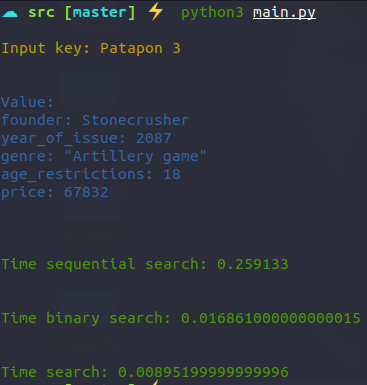
\includegraphics[width=1\textwidth]{res1.png}
		\caption{Результат работы программы}
		\label{ref:res1}}
\end{figure}

\begin{figure}[ht!]
	\centering{
		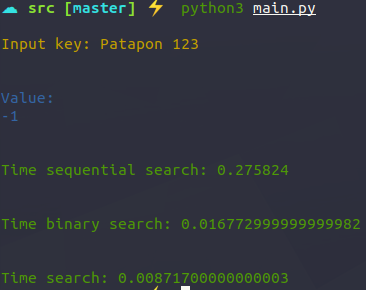
\includegraphics[width=1\textwidth]{res2.png}
		\caption{Результат работы программы}
		\label{ref:res2}}
\end{figure}


\begin{figure}[ht!]
	\centering{
		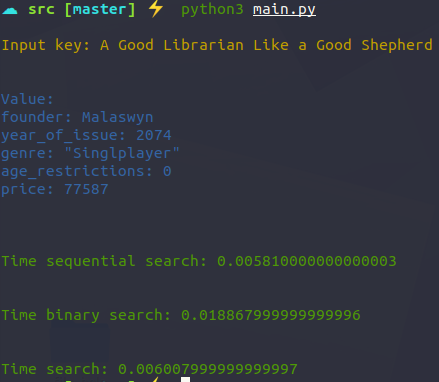
\includegraphics[width=0.7\textwidth]{res3.png}
		\caption{Результат работы программы}
		\label{ref:res3}}
\end{figure}


\newpage

\section{Параметризация муравьиного алгоритма}

В муравьином алгоритме вычисления производятся на основе настраиваемых параметров.

Рассмотрим матрицу смежностей размерностью $10\times10$ (\ref{table:matrix})

\begin{table}[ht]
	\centering
	\caption{Матрица смежностей}
	\label{table:matrix}
	\begin{tabular}{ | l | l | l | l | l | l | l | l | l | l | l |}
		\hline
		0 & 0    & 1    & 2    & 3    & 4    & 5    & 6    & 7    & 8    & 9    \\ \hline
		0 & 0    & 1790 & 200  & 1900 & 63   & 1659 & 1820 & 1395 & 2382 & 649  \\ \hline
		1 & 1790 & 0    & 1573 & 2435 & 1515 & 714  & 892  & 2193 & 1590 & 1003 \\ \hline
		2 & 200  & 1573 & 0    & 833  & 392  & 2404 & 962  & 902  & 141  & 1123 \\ \hline
		3 & 1900 & 2435 & 833  & 0    & 2283 & 1652 & 2362 & 2262 & 1512 & 2166 \\ \hline
		4 & 63   & 1515 & 392  & 2283 & 0    & 1322 & 290  & 1305 & 2100 & 969  \\ \hline
		5 & 1659 & 714  & 2404 & 1652 & 1322 & 0    & 256  & 78   & 2236 & 2041 \\ \hline
		6 & 1820 & 892  & 962  & 2362 & 290  & 256  & 0    & 1180 & 1547 & 1279 \\ \hline
		7 & 1395 & 2193 & 902  & 2262 & 1305 & 78   & 1180 & 0    & 1640 & 1161 \\ \hline
		8 & 2382 & 1590 & 141  & 1512 & 2100 & 2236 & 1547 & 1640 & 0    & 2212 \\ \hline
		9 & 649  & 1003 & 1123 & 2166 & 969  & 2041 & 1279 & 1161 & 2212 & 0    \\ \hline
	\end{tabular}
\end{table}

\newpage


\begin{table}[ht]
	\centering
	\caption{Таблица коэффициентов.Часть 1}
	\label{table:ref1}
	\begin{tabular}{ | l | l | l | l | l |}
		\hline
		$\alpha$ & $\beta$ & p   & Результат & Разница \\
		\hline
		0        & 1       & 0   & 6986      & 0       \\
		0        & 1       & 0.1 & 6986      & 0       \\
		0        & 1       & 0.2 & 6986      & 0       \\
		0        & 1       & 0.3 & 6986      & 0       \\
		0        & 1       & 0.4 & 6986      & 0       \\
		0        & 1       & 0.5 & 6986      & 0       \\
		0        & 1       & 0.6 & 6986      & 0       \\
		0        & 1       & 0.7 & 6986      & 0       \\
		0        & 1       & 0.8 & 6986      & 0       \\
		0        & 1       & 0.9 & 6992      & 6       \\
		0        & 1       & 1   & 6986      & 0       \\
		0.1      & 0.9     & 0   & 6986      & 0       \\
		0.1      & 0.9     & 0.1 & 6992      & 6       \\
		0.1      & 0.9     & 0.2 & 6986      & 0       \\
		0.1      & 0.9     & 0.3 & 6986      & 0       \\
		0.1      & 0.9     & 0.4 & 6986      & 0       \\
		0.1      & 0.9     & 0.5 & 6986      & 0       \\
		0.1      & 0.9     & 0.6 & 6986      & 0       \\
		0.1      & 0.9     & 0.7 & 6986      & 0       \\
		0.1      & 0.9     & 0.8 & 6986      & 0       \\
		0.1      & 0.9     & 0.9 & 7165      & 179     \\
		0.1      & 0.9     & 1   & 6986      & 0       \\
		0.2      & 0.8     & 0   & 6986      & 0       \\
		0.2      & 0.8     & 0.1 & 6986      & 0       \\
		0.2      & 0.8     & 0.2 & 6986      & 0       \\
		0.2      & 0.8     & 0.3 & 6992      & 6       \\
		0.2      & 0.8     & 0.4 & 6992      & 6       \\
		0.2      & 0.8     & 0.5 & 6992      & 6       \\
		0.2      & 0.8     & 0.6 & 6986      & 0       \\
		0.2      & 0.8     & 0.7 & 6992      & 6       \\
		0.2      & 0.8     & 0.8 & 6986      & 0       \\
		0.2      & 0.8     & 0.9 & 6986      & 0       \\
		0.2      & 0.8     & 1   & 6986      & 0       \\
		\hline
	\end{tabular}
\end{table}

\begin{table}[ht]
	\centering
	\caption{Таблица коэффициентов.Часть 2}
	\label{table:ref2}
	\begin{tabular}{ | l | l | l | l | l |}
		\hline
		$\alpha$ & $\beta$ & p   & Результат & Разница \\
		\hline
		0.3      & 0.7     & 0   & 6986      & 0       \\
		0.3      & 0.7     & 0.1 & 6986      & 0       \\
		0.3      & 0.7     & 0.2 & 7139      & 153     \\
		0.3      & 0.7     & 0.3 & 7139      & 153     \\
		0.3      & 0.7     & 0.4 & 6986      & 0       \\
		0.3      & 0.7     & 0.5 & 6986      & 0       \\
		0.3      & 0.7     & 0.6 & 6986      & 0       \\
		0.3      & 0.7     & 0.7 & 6986      & 0       \\
		0.3      & 0.7     & 0.8 & 6992      & 6       \\
		0.3      & 0.7     & 0.9 & 6992      & 6       \\
		0.3      & 0.7     & 1   & 6986      & 0       \\
		0.4      & 0.6     & 0   & 6986      & 0       \\
		0.4      & 0.6     & 0.1 & 6992      & 6       \\
		0.4      & 0.6     & 0.2 & 6986      & 0       \\
		0.4      & 0.6     & 0.3 & 6986      & 0       \\
		0.4      & 0.6     & 0.4 & 6986      & 0       \\
		0.4      & 0.6     & 0.5 & 6992      & 6       \\
		0.4      & 0.6     & 0.6 & 6992      & 6       \\
		0.4      & 0.6     & 0.7 & 6986      & 0       \\
		0.4      & 0.6     & 0.8 & 7139      & 153     \\
		0.4      & 0.6     & 0.9 & 6986      & 0       \\
		0.4      & 0.6     & 1   & 6992      & 6       \\
		0.5      & 0.5     & 0   & 7139      & 153     \\
		0.5      & 0.5     & 0.1 & 6986      & 0       \\
		0.5      & 0.5     & 0.2 & 6986      & 0       \\
		0.5      & 0.5     & 0.3 & 7139      & 153     \\
		0.5      & 0.5     & 0.4 & 6986      & 0       \\
		0.5      & 0.5     & 0.5 & 6986      & 0       \\
		0.5      & 0.5     & 0.6 & 6986      & 0       \\
		0.5      & 0.5     & 0.7 & 6986      & 0       \\
		0.5      & 0.5     & 0.8 & 6986      & 0       \\
		0.5      & 0.5     & 0.9 & 6986      & 0       \\
		0.5      & 0.5     & 1   & 6986      & 0       \\

		\hline
	\end{tabular}
\end{table}


\begin{table}[ht]
	\centering
	\caption{Таблица коэффициентов.Часть 3}
	\label{table:ref3}
	\begin{tabular}{ | l | l | l | l | l |}
		\hline
		$\alpha$ & $\beta$ & p   & Результат & Разница \\
		\hline
		0.6      & 0.4     & 0   & 7139      & 153     \\
		0.6      & 0.4     & 0.1 & 6992      & 6       \\
		0.6      & 0.4     & 0.2 & 6986      & 0       \\
		0.6      & 0.4     & 0.3 & 6986      & 0       \\
		0.6      & 0.4     & 0.4 & 7139      & 153     \\
		0.6      & 0.4     & 0.5 & 6992      & 6       \\
		0.6      & 0.4     & 0.6 & 6986      & 0       \\
		0.6      & 0.4     & 0.7 & 6986      & 0       \\
		0.6      & 0.4     & 0.8 & 6986      & 0       \\
		0.6      & 0.4     & 0.9 & 6992      & 6       \\
		0.6      & 0.4     & 1   & 6986      & 0       \\
		0.7      & 0.3     & 0   & 6986      & 0       \\
		0.7      & 0.3     & 0.1 & 6986      & 0       \\
		0.7      & 0.3     & 0.2 & 6986      & 0       \\
		0.7      & 0.3     & 0.3 & 7139      & 153     \\
		0.7      & 0.3     & 0.4 & 7165      & 179     \\
		0.7      & 0.3     & 0.5 & 7139      & 153     \\
		0.7      & 0.3     & 0.6 & 6992      & 6       \\
		0.7      & 0.3     & 0.7 & 6992      & 6       \\
		0.7      & 0.3     & 0.8 & 6986      & 0       \\
		0.7      & 0.3     & 0.9 & 6992      & 6       \\
		0.7      & 0.3     & 1   & 6986      & 0       \\
		0.8      & 0.2     & 0   & 7139      & 153     \\
		0.8      & 0.2     & 0.1 & 7562      & 576     \\
		0.8      & 0.2     & 0.2 & 6992      & 6       \\
		0.9      & 0.1     & 0.2 & 6992      & 6       \\
		0.9      & 0.1     & 0.3 & 6986      & 0       \\
		0.9      & 0.1     & 0.4 & 7139      & 153     \\
		0.9      & 0.1     & 0.5 & 7329      & 343     \\
		0.9      & 0.1     & 0.6 & 7217      & 231     \\
		0.9      & 0.1     & 0.7 & 7139      & 153     \\
		0.9      & 0.1     & 0.8 & 7217      & 231     \\
		0.9      & 0.1     & 0.9 & 7376      & 390     \\
		0.9      & 0.1     & 1   & 6986      & 0       \\
		\hline
	\end{tabular}
\end{table}


\begin{table}[ht]
	\centering
	\caption{Таблица коэффициентов.Часть 4}
	\label{table:ref4}
	\begin{tabular}{ | l | l | l | l | l |}
		\hline
		$\alpha$ & $\beta$ & p   & Результат & Разница \\
		\hline
		1        & 0       & 0   & 8531      & 1545    \\
		1        & 0       & 0.1 & 8588      & 1602    \\
		1        & 0       & 0.2 & 6986      & 0       \\
		1        & 0       & 0.3 & 7720      & 734     \\
		1        & 0       & 0.4 & 7554      & 568     \\
		1        & 0       & 0.5 & 6992      & 6       \\
		1        & 0       & 0.6 & 7920      & 934     \\
		1        & 0       & 0.7 & 7217      & 231     \\
		1        & 0       & 0.8 & 7874      & 888     \\
		1        & 0       & 0.9 & 7446      & 460     \\
		1        & 0       & 1   & 8119      & 1133    \\
		\hline
	\end{tabular}
\end{table}

\newpage

Параметризация метода решения задачи коммивояжера
на основании муравьиного алгоритма проводилась для матрицы с
элементами в диапозоне [0, 2500].
Количество дней было равно 50.
Полный перебор определил оптимальную длину пути 6986.
Столбец ''результат'' отвечает за результат работы муравьиного алгоритма.
Столбец ''разница'' отвечает за разницу с оптимальной длиной.




\section{Вывод}

На основе проведенной параметризации (таблицы \ref{table:ref1}--\ref{table:ref4}) для матрицы смежности
приведенной в таблице (\ref{table:matrix}) рекомендуется использовать
$(\alpha = 0.5, \beta = 0.5, \rho = \text{любое})$.
При этих параметрах, количество правильно найденных оптимальных путей составило 8 единиц.

% В данном разделе было произведено сравнение
% последовательной реализации трех алгоритмов
% и конвейера с использованием многопоточности.
% По результатам исследования конвейерную обработку
% нет смысла применять на задачах, занимающих мало времени.
% Статистика показала, что конвейерная обработка работает правильно.


\backmatter %% Здесь заканчивается нумерованная часть документа и начинаются ссылки и
%% заключение

\chapter*{Заключение}
\addcontentsline{toc}{chapter}{Заключение}

В данной лабораторной работе были рассмотрены
основополагающие материалы которые в дальнейшем потребовались
при реализации алгоритма полного перебора и муравьиного алгоритма.
Были рассмотрены схемы (рис. \ref{ref:d0}--\ref{ref:d1})
для решения задачи коммивояжера.
Также были разобраны листинги 3.1-3.2,
показывающие работу, описанных выше, алгоритмов и были приведены рисунки
\ref{ref:res1} - \ref{ref:res3},
показывающий работу алгоритмов.
Был произведен сравнительный анализ рис. \ref{ref:time}.


В рамках выполнения работы решены следующие задачи:


\begin{enumerate}
	\item изучены два алгоритма для решения задачи коммивояжера;
	\item применены изученные основы для реализации двух алгоритмов;
	\item получены практические навыки;
	\item проведена параметризация муравьиного алгоритма;
	\item проведен сравнительный анализ скорости работы реализованных алгоритмов;
	\item описан и обоснован выбор язык программирования, для решения поставленной задачи.
\end{enumerate}

\addcontentsline{toc}{chapter}{Список литературы}
\begin{thebibliography}{3}
	\bibitem{Vs}
	Visual Studio Code [Электронный ресурс], режим доступа: https://code.visualstudio.com/ (дата обращения: 02.10.2020)
	\bibitem{Win}
	Windows [Электронный ресурс], режим доступа:https://www.microsoft.com/ru-ru/windows (дата обращения: 02.10.2020)
	\bibitem{Lin}
	Linux [Электронный ресурс], режим доступа:https://www.linux.org.ru/ (дата обращения: 02.10.2020)
	\bibitem{Microsoft}
	Справочник по языку C [Электронный ресурс], режим доступа:https://docs.microsoft.com/ru-ru/cpp/c-language/c-language-reference?view=msvc-160 (дата обращения: 25.12.2020)
	\bibitem{Ubuntu}
	Ubuntu 18.04 [Электронный ресурс], режим доступа:https://releases.ubuntu.com/18.04/ (дата обращения: 02.10.2020)
\end{thebibliography}


%\appendix   % Тут идут приложения

\end{document}